% Document class and language
\documentclass{article}
\usepackage{polski}
\usepackage[square,numbers]{natbib}
\bibliographystyle{unsrtnat}

% Setting geometry
\usepackage[a4paper,top=2cm,bottom=2cm,left=3cm,right=3cm,marginparwidth=1.75cm]{geometry}

% Useful packages
\newcommand{\pyobject}[1]{\texttt{#1}}
\usepackage{csvsimple}
\usepackage{graphicx}

\title{Analiza zależności wyników drużyny piłkarskiej w lidze od wybranych statystyk drużynowych}
\author{Daniel Borkowski, 266593}
\date{5 czerwca 2023 r.}
\renewcommand\refname{Źródła}

\begin{document}
\maketitle
\tableofcontents

\section{Wstęp}

\subsection{Cel}
Celem projektu jest \textbf{znalezienie, zbadanie i opisanie zależności} wyników drużyny piłkarskiej w lidze od wybranych mniej lub bardziej oczywistych statystyk drużynowych w celu \textbf{budowy modelu} przewidującego jak dobrze radzi sobie dana drużyna w lidze na podstawie tych statystyk. Ze względu na wybór czynników podzielimy to zadanie na dwie niezależne części:
\begin{enumerate}
    \item przewidywanie na podstawie bardziej oczywistych czynników (model \textit{łatwy}):
    \begin{enumerate}
        \item ilości goli strzelonych
        \item ilości goli straconych
    \end{enumerate}
    \item przewidywanie na podstawie mniej oczywistych czynników (model \textit{trudny}):
    \begin{enumerate}
        \item udział młodych zawodników w grze zespołu
        \item udział zagranicznych zawodników w grze zespołu
    \end{enumerate}
\end{enumerate}

Czynnikiem w piłce nożnej, który określa wynik drużyny jest natomiast liczba zdobytych przez nią \textbf{punktów}.
Definiujemy zatem nasz cel nieco bardziej szczegółowo, jako analizę zależności między \textbf{bramkami} strzelonymi i straconymi przez drużynę, a jej punktami w sezonie oraz analizę zależności między \textbf{strukturą składu drużyny}, a jej punktami w sezonie.

\subsection{Plan}
\paragraph{}
Skupimy się na naszym krajowym podwórku i rozgrywkach Ekstraklasy \cite{ekstraklasa}. Za zgodą administratorów portalu EkstraStats \cite{ekstrastats} wykorzystamy dostępne tam dane na temat rozgrywek w latach 2015-2022. Nie wykorzystamy danych z sezonu 2014/2015 oraz 2022/2023 ze względu na ich niekompletność. Pozyskamy następujące metryki dla każdej drużyny w każdym sezonie:
\begin{enumerate}
    \item liczba rozegranych meczów
    \item liczba straconych bramek
    \item liczba strzelonych bramek
    \item liczba zdobytych punktów
    \item liczba minut rozegranych przez młodzieżowców
    \item liczba goli zdobytych przez młodzieżowców
    \item liczba minut rozegranych przez zagranicznych zawodników
    \item liczba goli zdobytych przez zagranicznych zawodników
\end{enumerate}
Umożliwi nam to realizację celu na podstawie 114 rekordów występów drużyn w rozgrywkach ligowych.

\section{Dane}

\subsection{Pozyskanie danych}

Strona \cite{ekstrastats} udostępnia wiele ciekawych danych na temat rozgrywek ligowych, zawierających się w kilkudziesięciu tabelach dla każdego sezonu. Ograniczymy się do interesujących nas informacji: tabel ligowych, tabel młodzieżowców i tabel zawodników zagranicznych. 

Używając skryptu \pyobject{scrapping.py} dokonujemy zatem ekstrahowania interesujących nas tabel ze strony. Dane są zbierane hobbystów i na tym etapie natrafiamy na pewne problemy, jakim jest niespójność w ich zapisie: \textit{klucze}, które zaraz będą potrzebne do łączenia danych nie są bowiem jednolite nawet dla różnych tabel w tym samym sezonie. Co więcej, ta niespójność nie jest konsekwentna i tak jak raz tę samą drużynę określa się jako \textit{Wisła Kraków} i \textit{Wisła K.}, tak czasem \textit{Termalicę} w innej tabeli reprezentuje \textit{Bruk-Bet}. Nie uciekniemy tu zatem od ręcznej korekty kluczy w pobranych plikach \pyobject{.csv}. 

Dopiero po tym kroku możemy przejść do dalszych działań, jakimi są połączenie tabel dla danych sezonów i odrzucenie kolumn, którymi nie jesteśmy zainteresowani, jak na przykład \textit{liczba porażek}, czy też \textit{procent goli drużyny zdobytych przez zagranicznych zawodników}, którą to metrykę możemy obliczyć. Na koniec otrzymujemy 7 tabel zawierających w sumie 114 rekordów ośmiu metryk wymienionych powyżej oraz kolumnę \textit{KLUB} będącą kluczem używanym w celu łączenia danych i kolumnę \textit{season} informującą o sezonie, w którym odbyły się rozgrywki.

\subsection{Analiza danych}

Pozyskane dane dla różnych sezonów łączymy i zaczynamy analizę. Wykorzystamy narzędzia oferowane przez \pyobject{y\_data\_profiling} oraz przyjrzymy się ręcznie pozyskanym tabelom. Poniżej w tabeli \ref{tab:head} pięć początkowych rekordów i kolejno ich indeks, liczba rozegranych meczów, zdobytych punktów, strzelonych bramek, straconych bramek, minut i strzelonych bramek obcokrajowców, minut i strzelonych bramek młodzieżowców oraz sezonu.
\begin{table}[h!]
\centering
\caption{Efekt wywołania metody \pyobject{head} na zebranych danych}
\label{tab:head}
\csvreader[
    tabular=|c|c|c|c|c|c|c|c|c|c|,
    no head,
    table head=\hline id & played & points & gf & ga & fm & fg & ym & yg & season \\ \hline,
    late after last line=\\\hline
]{head.csv}{}
{\csvcoli & \csvcolii & \csvcoliii & \csvcoliv & \csvcolv & \csvcolvi & \csvcolvii & \csvcolviii & \csvcolix & \csvcolx}
\end{table}

Ze względu na sposób i źródło pozyskanych danych w tabeli nie ma brakujących wartości. 

\begin{table}[h!]
\centering
\caption{Mediany wartości dla poszczególnych sezonów}
\label{tab:groups}
\csvreader[
    tabular=|c|c|c|c|c|c|c|c|c|,
    no head,
    table head=\hline season & played & points & gf & ga & fm & fg & ym & yg \\ \hline,
    late after last line=\\\hline
]{groups.csv}{}
{\csvcoli & \csvcolii & \csvcoliii & \csvcoliv & \csvcolv & \csvcolvi & \csvcolvii & \csvcolviii & \csvcolix}
\end{table}

Jednakże, dokonując grupowania natrafiamy na inny problem potencjalnie rzutujący na późniejsze wyniki. W różnych sezonach, co widzimy na tabeli \ref{tab:groups}, różnie kształtowały się mediany poszczególnych wartości. Przyczyny tego zjawiska korzystając z własnej wiedzy na temat rozgrywek Ekstraklasy i dodatkowych materiałów \cite{przepis} diagnozujemy następująco:
\begin{itemize}
    \item \textbf{zmiana formuły rozgrywek} - co widoczne po różnej liczbie rozegranych meczów, rozgrywki w badanym okresie kilkukrotnie zmieniały format
    \item \textbf{zmiana innych przepisów} - w 2019 roku wprowadzono obowiązek gry młodzieżowca w każdym meczu
    \item \textbf{zmiana znaczenia wartości kolumn} - nierozwiane dotychczas wątpliwości na temat znaczenia słowa \textit{młodzieżowiec} warto rozwiać - na przestrzeni różnych sezonów zmieniał się sposób pojmowania takich zawodników, najpierw jako piłkarzy poniżej 24. roku życia, a potem 21.
\end{itemize}

\begin{figure}[h!]
    \centering
    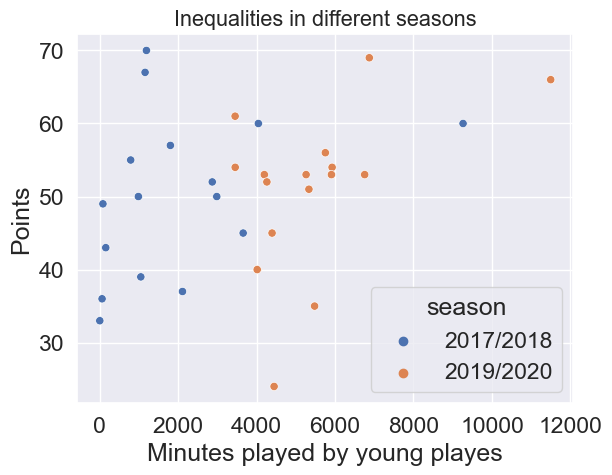
\includegraphics[width=0.75\textwidth]{min_by_sea.png}
    \caption{Zależność liczby punktów zdobytych przez drużynę od liczby minut rozegranych przez młodzieżowców.}
    \label{fig:min_by_sea}
\end{figure}

Warto więc odwołać się do czynników, które się nie zmieniają. Oprócz tego, że parafrazując legendarnego polskiego trenera Kazimierza Górskiego, \textit{piłka zawsze była jedna, a bramki zawsze były dwie}, nie zmieniły się najważniejsze zasady meczów piłkarskich. W każdym z rozgrywanych meczów do zdobycia były trzy punkty za zwycięstwo i jeden punkt za remis, a każda bramka liczyła się tak samo. Odpowiada nam to na zmianę formuły rozgrywek, ale nie rozwiązuje kwestii zmiany przepisów i zmiany znaczenia wartości kolumn. Nie chcąc rezygnować z pozyskanych metryk (wobec braku dostępnych lepszych danych) proponujemy standaryzację wartości dla poszczególnych sezonów.

\begin{table}[h!]
\centering
\caption{Odchylenia standardowe wartości dla poszczególnych sezonów}
\label{tab:groups_std}
\csvreader[
    tabular=|c|c|c|c|c|c|c|c|c|,
    no head,
    table head=\hline season  & points & gf & ga & fm & fg & ym & yg \\ \hline,
    late after last line=\\\hline
]{groups_std.csv}{}
{\csvcoli & \csvcolii & \csvcoliii & \csvcoliv & \csvcolv & \csvcolvi & \csvcolvii & \csvcolviii}
\end{table}

\begin{figure}[h!]
    \centering
    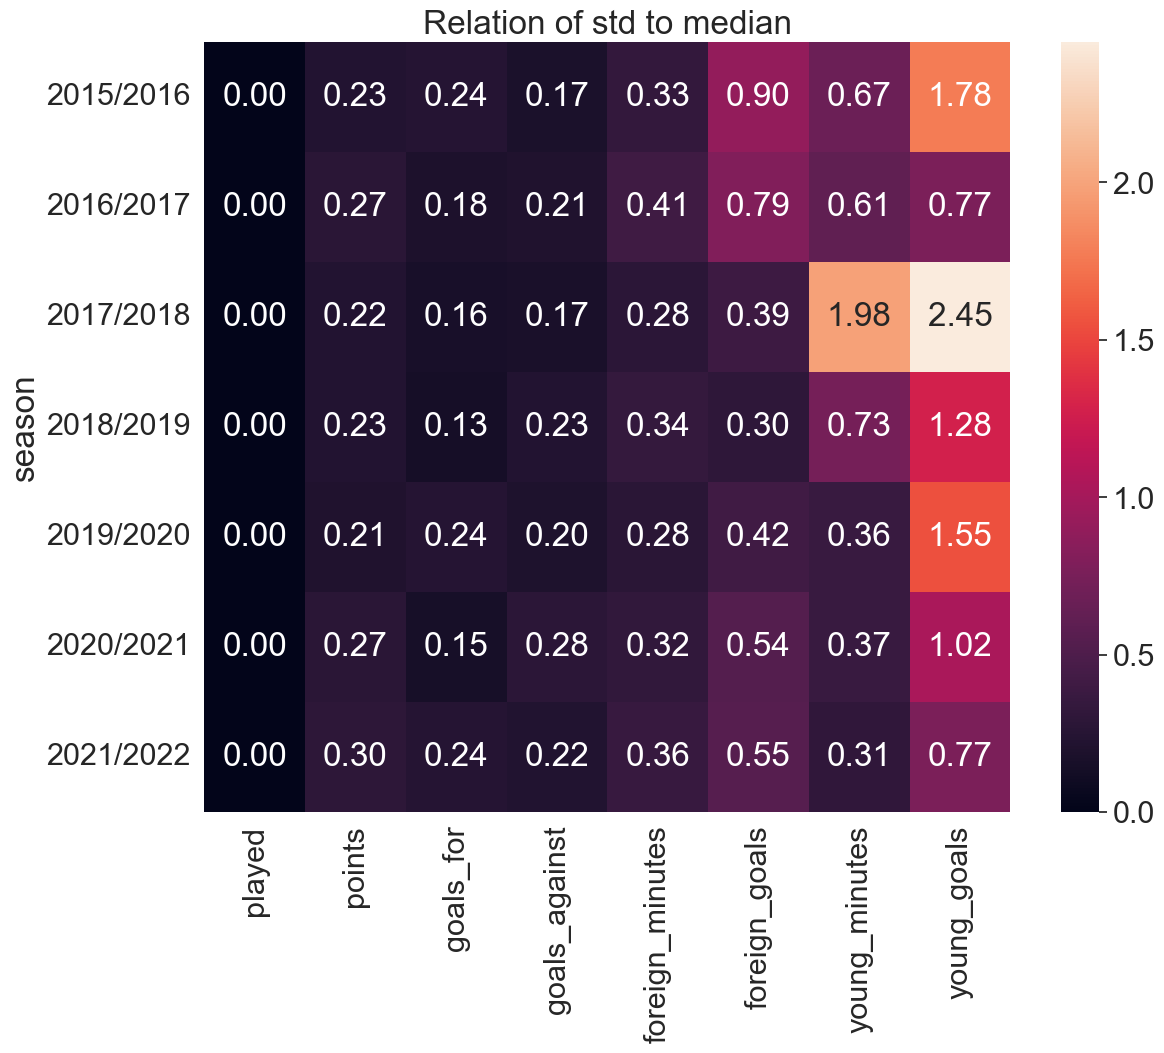
\includegraphics[width=0.75\textwidth]{std_to_med.png}
    \caption{Stosunek odchylenia standardowego do mediany dla poszczególnych sezonów}
    \label{fig:std_to_med}
\end{figure}

Po zbadaniu odchylenia standardowego na tabeli \ref{tab:groups_std} i jego stosunku do mediany na grafice \ref{fig:std_to_med} podejmujemy decyzję o zastosowaniu standaryzacji względem mediany, gdyż jest ona mniej podatna na skrajne wartości, których, zwłaszcza w kolumnach dotyczących młodych graczy, nie brakuje, co widać na grafice \ref{fig:min_by_sea}, gdzie widoczne jest także wprowadzenie obowiązku gry młodzieżowca w sezonie 2019/2020.

Proponujemy zatem uzależnienie wszystkich wartości od liczby rozegranych meczów w sezonie, uzależnienie zdobywanych przez zawodników goli od goli drużyny oraz wstępną standaryzację wartości dotyczących piłkarzy młodzieżowych i zagranicznych, tak aby otrzymane wskaźniki wyrażały ogólnie \textit{czy klub stawia na młodzieżowców}, \textit{czy bramki zespołu są zdobywane przez zagranicznych zawodników} i były niezależne od trendu w danym sezonie spowodowanego przepisami lub innymi czynnikami zewnętrznymi.

Przetworzone w ten sposób dane poddamy właściwej analizie w celu stworzenia modelu.


\subsection{Przetwarzanie danych}

Dokonujemy zatem transformacji danych, chcąc uzyskać następujące wskaźniki:

\begin{itemize}
    \item \textbf{liczba punktów drużyny na mecz} - główny wskaźnik sukcesu bądź porażki drużyny, będziemy go przewidywać
    \item \textbf{liczba goli zdobytych i straconych na mecz} - podstawowe wskaźniki, z użyciem których będziemy przewidywać liczbę punktów na mecz
    \item \textbf{wskaźnik minut młodzieżowców} - oddanie skłonności drużyny do grania młodymi zawodnikami
    \item  \textbf{wskaźnik udziału młodzieżowców w golach zespołu} - oddanie rzeczywistego znaczenia młodych zawodników w drużynie
    \item \textbf{wskaźnik minut zawodników zagranicznych} - oddanie skłonności drużyny do grania zawodnikami zza granicy
    \item  \textbf{wskaźnik udziału zawodników zagranicznych w golach zespołu} - oddanie rzeczywistego znaczenia zawodników zagranicznych w drużynie
\end{itemize}

Warto zaznaczyć, że używane słowo \textit{wskaźnik}, nomen omen, \textit{wskazuje} na wysoki poziom przetworzenia danych - na tym etapie nie mają już bezpośredniego przełożenia na rzeczywistość, jedynie oddają skłonności i trendy, na czym - w kontekście celu projektu - nam zależy.

\begin{table}[h!]
\centering
\caption{Wartości mediany dla poszczególnych sezonów po transformacji}
\label{tab:groups_transformed}
\csvreader[
    tabular=|c|c|c|c|c|c|c|c|,
    no head,
    table head=\hline season & points & gf & ga & fm & fg & ym & yg \\ \hline,
    late after last line=\\\hline
]{groups_transformed.csv}{}
{\csvcoli & \csvcolii & \csvcoliii & \csvcoliv & \csvcolv & \csvcolvi & \csvcolvii & \csvcolviii}
\end{table}

Po przeprowadzeniu transformacji mediany nierówności zostały usunięte. Na rysunku \ref{fig:min_by_sea_trans} nie widzimy znaczących różnic pomiędzy danymi dla sezonów sprzed i po wprowadzeniu przepisu o obowiązku grania młodzieżowca w każdym meczu. Tak przetworzone dane możemy analizować pod kątem stworzenia modelu.

\begin{figure}[h!]
    \centering
    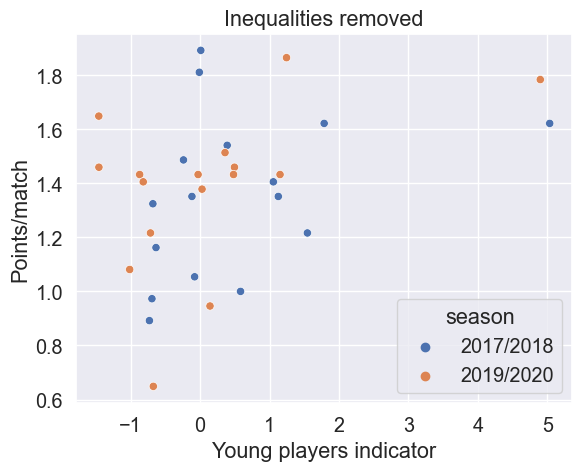
\includegraphics[width=0.75\textwidth]{min_by_sea_trans.png}
    \caption{Zależność liczby punktów zdobytych przez drużynę na mecz od tego ile w zespole rozegrali młodzi zawodnicy.}
    \label{fig:min_by_sea_trans}
\end{figure}

\subsection{Analiza przetworzonych danych}

Poszukujemy zależności między poszczególnymi metrykami korzystając z macierzy korelacji na rysunku \ref{fig:corr}.

\begin{figure}[h!]
    \centering
    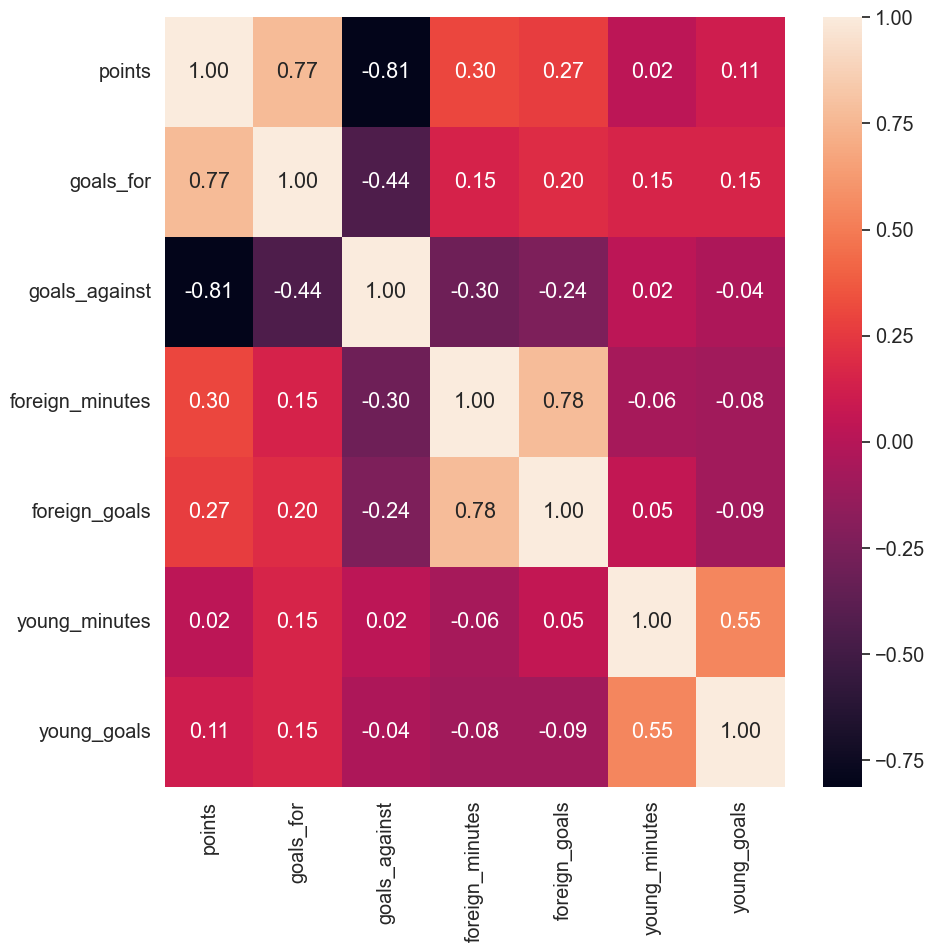
\includegraphics[width=0.75\textwidth]{corr_mat.png}
    \caption{Macierz korelacji.}
    \label{fig:corr}
\end{figure}

Skupiając się na celu przedsięwzięcia przyglądamy się poszczególnym metrykom i im zależnościom względem metryki \textit{points}.

\begin{figure}[h!]
    \centering
    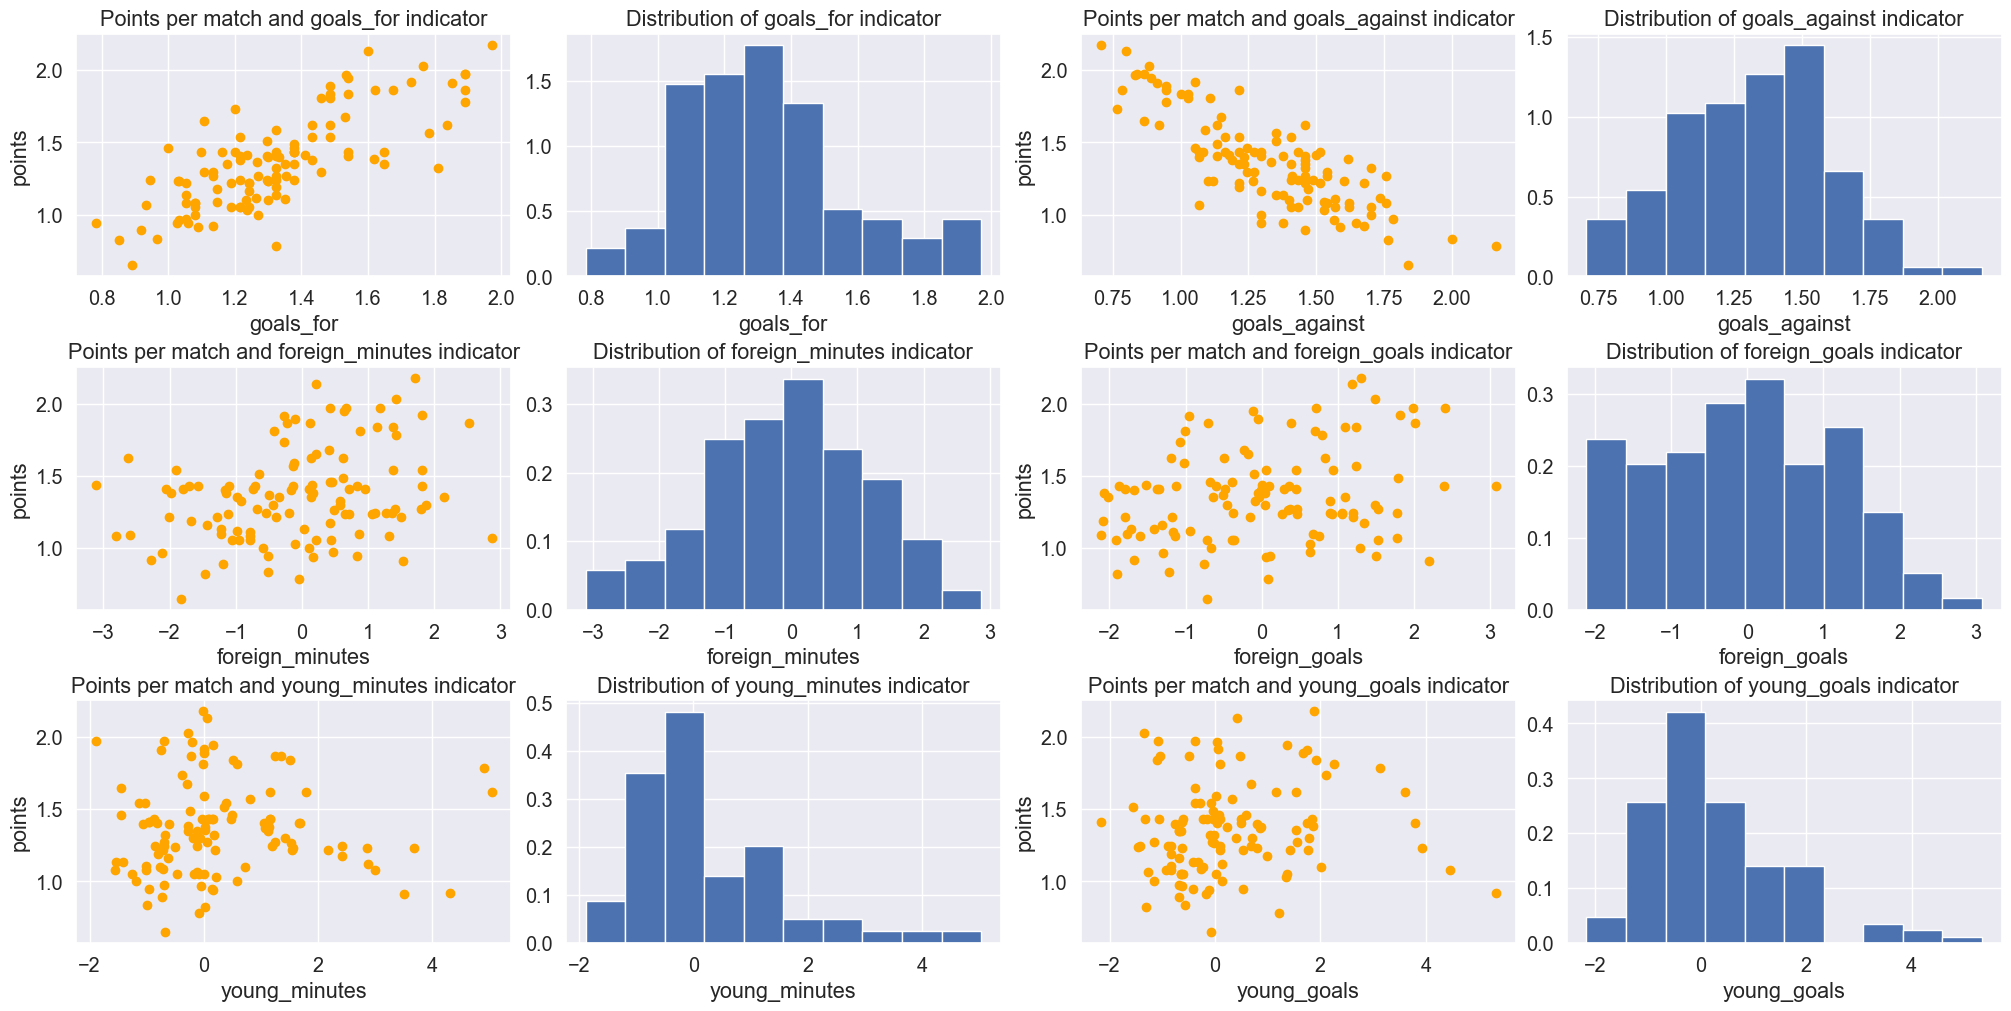
\includegraphics[width=1\textwidth]{dependencies.png}
    \caption{Zależności między metrykami a punktami na mecz.}
    \label{fig:dependencies}
\end{figure}

Na podstawie uzyskanych wykresów możemy wysnuć następujące wnioski:
\begin{itemize}
    \item mniej oczywiste metryki są słabo zależne względem punktów:
    \begin{itemize}
            \item uzyskane wskaźniki dotyczące młodzieżowców są bardzo słabo zależne względem wszystkich innych metryk
            \item uzyskane wskaźniki dotyczące młodzieżowców są silnie skupione wokół średnich wartości
            \item uzyskane wskaźniki dotyczące zawodników zza granicy są słabo zależne względem punktów
    \end{itemize}
    \item bardziej oczywiste metryki są silnie zależne względem punktów
\end{itemize}

Przeprowadzona dogłębna analiza posłuży nam jako uzasadnienie wniosków uzyskanych w eksperymencie.

\section{Modele}

\subsection{Narzędzia}

W budowie modelu będziemy wykorzystywać narzędzia dostarczane przez pakiet \pyobject{scikit-learn}:
\begin{itemize}
    \item model: maszyna wektorów nośnych do regresji liniowej
    \item metryka: średni błąd bezwzględny (o wzorze \ref{eq:mae})
    \item preprocessing: \pyobject{StandardScaler}
    \item inne narzędzia: \pyobject{train\_test\_split}, \pyobject{GridSearchCV}
\end{itemize}

\subsection{Dobór parametrów}

Wykorzystując \pyobject{GridSearchCV} na podstawie wartości \pyobject{mean\_absolute\_error} i danych treningowych poszukujemy najlepszego modelu, spośród następujących wartości:
\begin{itemize}
    \item \textbf{kernel}, jądro wskazujące zastosowany typ regresji liniowej - \textit{linear}, \textit{poly}, \textit{rbf}
    \item \textbf{C}, wskaźnik regularyzacji (uproszczenia) - 1, 2, 5, 10, 15
    \item \textbf{gamma}, parametr jądra - 000.1, 000.5, 0.01, 0.05, 0.1, 1
\end{itemize}

Poszukiwania określają optymalne wartości tych parametrów jako: \textit{c=2, gamma=0.05, kernel=rbf} dla modelu przewidującego na podstawie danych dotyczących młodzieżowców i piłkarzy zza granicy oraz \textit{c=15, gamma=0.01, kernel=rbf} dla modelu przewidującego na podstawie goli strzelonych i straconych.

\subsection{Wyniki}

\begin{figure}[h!]
    \centering
    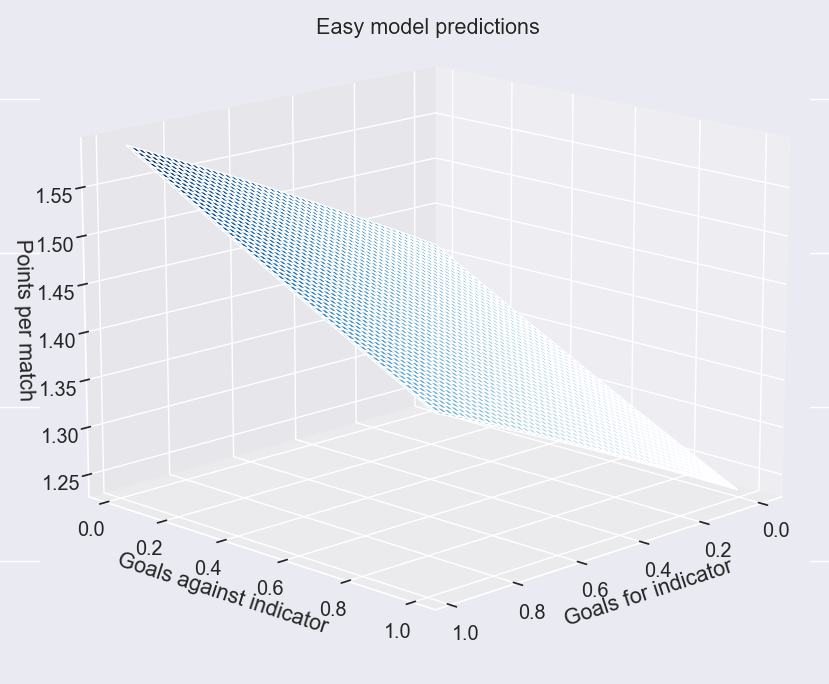
\includegraphics[width=0.75\textwidth]{3d.png}
    \caption{Wykres przewidywań dla różnych wartości czynników goli strzelonych i straconych (model \textit{łatwy})}
    \label{fig:3d}
\end{figure}

Otrzymane wyniki będziemy odnosić do średniego odchylenia bezwzględnego (medianowego), ze względu na analogiczny sposób jego obliczenia do używanego w modelu średniego błędu bezwzględnego, gdzie występuje analogia między różnicą wartości i mediany, a różnicą wartości i wartości przewidywanej przez model. Wartość średniego odchylenia bezwzględnego dla rubryki \textit{punkty na mecz} to \textbf{0.25}.

\begin{equation}\label{eq:mad}
MAD={\frac{1}{N}\sum\limits_{i=1}^N |x_i - m(X)|}
\end{equation}

\begin{equation}\label{eq:mae}
MAE={\frac{1}{N}\sum\limits_{i=1}^N |x_i - y_i|}
\end{equation}

Dla modelu \textit{nieoczywistego} średni błąd bezwzględny wynosi \textbf{0.29}, natomiast dla modelu \textit{oczywistego} - \textbf{0.10}.

Na tej podstawie należy stwierdzić, że \textbf{przewidywanie wyników drużyny na podstawie udziału w grze młodzieżowców i zawodników zza granicy jest obarczone dużym błędem}, a model \textit{trudniejszy} radzi sobie znacznie gorzej niż \textit{prostszy}.

Działanie \textit{prostszego} z modeli widoczne jest na rysunku \ref{fig:3d}. Zgodnie z intuicją, drużyna radzi sobie lepiej jeśli traci mniej goli i strzela więcej goli.



\subsection{Eksperyment}

Żeby ostatecznie ocenić jakość otrzymanych modeli przeprowadzimy eksperyment na danych z aktualnego sezonu. Nie są one pełne, brakuje ostatniej serii gier, jednakże dla naszych modeli nie stanowi to żadnego problemu. Wyniki drużyn w tym sezonie widoczne są w tabeli \ref{tab:tab22}.

\begin{table}[h!]
\centering
\caption{Tabela ligowa w sezonie 2022/2023 po 33 spotkaniach}
\label{tab:tab22}
\csvreader[
    tabular=|c|c|c|,
    no head,
    table head=\hline id & klub & punkty \\ \hline,
    late after last line=\\\hline
]{tab22.csv}{}
{\csvcolii & \csvcoliii & \csvcoliv}
\end{table}

\subsubsection{Model trudny}

\begin{table}[h!]
\centering
\caption{Predykcja punktów po 33 meczach na podstawie udziału w grze zespołu młodzieżowców i zawodników zza granicy w porównaniu do stanu faktycznego z tabeli \ref{tab:tab22}}
\label{tab:tab22_hard}
\csvreader[
    tabular=|c|c|c|c|c|c|c|c|c|,
    no head,
    table head=\hline id & +/- & klub & punkty & +/- & fm & fg & ym & yg \\ \hline,
    late after last line=\\\hline
]{tab_22_hard.csv}{}
{\csvcolii & \csvcoliii & \csvcoliv & \csvcolv & \csvcolvi & \csvcolvii & \csvcolviii & \csvcolix & \csvcolx}
\end{table}

W tabeli \ref{tab:tab22_hard} widoczne są przewidywania modelu \textit{trudnego}. Jest kilka sukcesów (ostatnia Miedź, czołowe trzy zespoły są wysoko) i kilka spektakularnych porażek (czwarta Pogoń druga od końca).

W sumie model pomylił się o 84 miejsca w tabeli (średnio 4.67 na drużynę) i 162 punkty (9 na drużynę). Na wykresach zamieszczonych na rysunku \ref{hard_dep:3d} widać pewne próby \textbf{dopasowania modelu do wskaźnika minut rozegranych przez piłkarzy zagranicznych, które nie zawsze przynosiły oczekiwany efekt}. Jest to przyczyną niedoszacowania Pogoni, która mniej stawiała na zagranicznych graczy od innych zespołów z czołówki. 

Największą \textbf{premię} dostały Piast i Cracovia, zapewne w związku z dużą bramkostrzelnością graczy zagranicznych i, w odróżnieniu od Jagielloni, pewną bramkostrzelnością młodzieżowców.

\begin{figure}[h!]
    \centering
    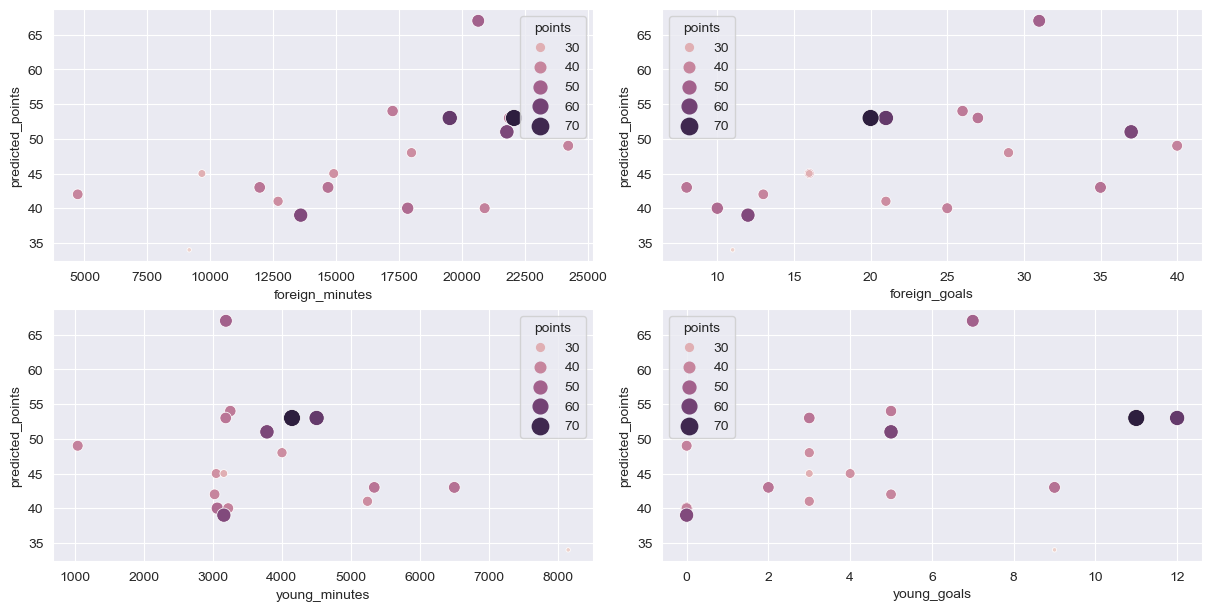
\includegraphics[width=1\textwidth]{hard_model_dependencies.png}
    \caption{Zależności przewidywań modelu \textit{trudnego} od poszczególnych wskaźników}
    \label{hard_dep:3d}
\end{figure}

\subsubsection{Model prosty}

\begin{table}[h!]
\centering
\caption{Predykcja punktów po 33 meczach na podstawie strzelonych i straconych goli w porównaniu do stanu faktycznego z tabeli \ref{tab:tab22}}
\label{tab:tab22_easy}
\csvreader[
    tabular=|c|c|c|c|c|c|c|,
    no head,
    table head=\hline id & +/- & klub & punkty & +/- & gf & ga \\ \hline,
    late after last line=\\\hline
]{tab22_easy.csv}{}
{\csvcolii & \csvcoliii & \csvcoliv & \csvcolv & \csvcolvi & \csvcolvii & \csvcolviii}
\end{table}


\begin{figure}[h!]
    \centering
    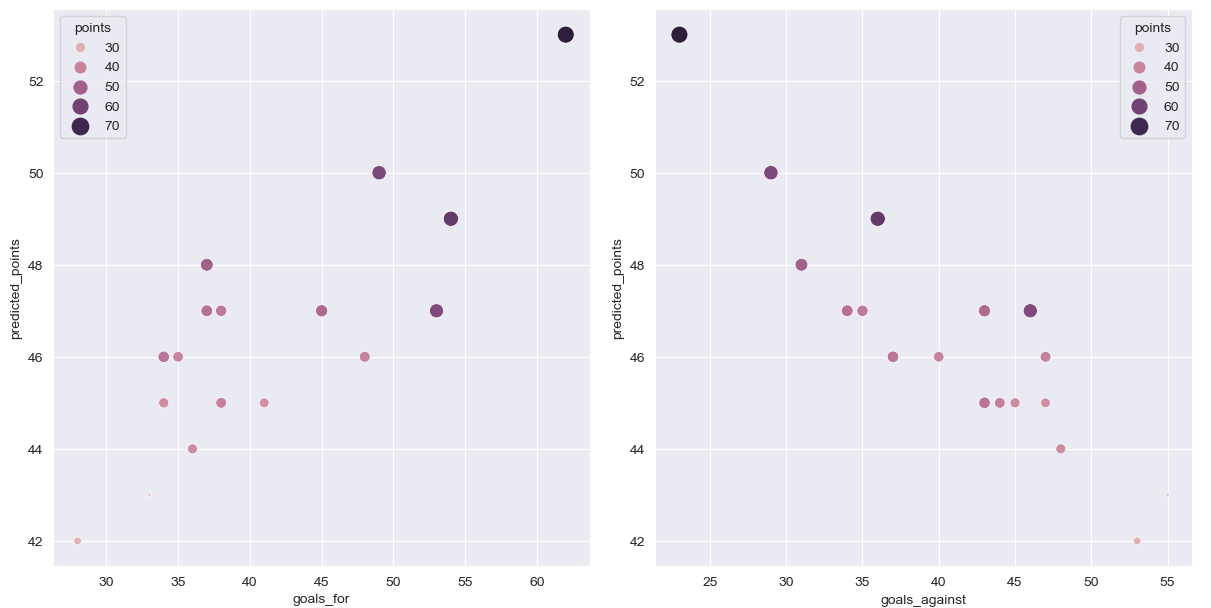
\includegraphics[width=1\textwidth]{easy_model_dependencies.png}
    \caption{Zależności przewidywań modelu \textit{łatwego} od poszczególnych wskaźników}
    \label{easy_dep:3d}
\end{figure}

Przewidywania wyników drużyny na podstawie bramek strzelonych i straconych widoczne są w w tabeli \ref{tab:tab22_easy}. 

W sumie model pomylił się o 30 (robi wrażenie w porównaniu do poprzednich 84) miejsc w tabeli i 131 punktów uprzednio (162). Przyczyny takiego dysonansu można upatrywać w doborze metryki - 
\textit{punktów na mecz} - jako pewnego wskaźnika sukcesu. Z punktu widzenia postawionych celów dobre umiejscowienie drużyn w tabeli jest zatem bardziej znaczące niż słabe przewidywania punktów na mecz, ze względu na ograniczenia tej rubryki. 

Można powiedzieć, że model szukał balansu między ofensywą, a defensywą. Widoczne są silnie liniowe zależności, na co wskazywała już wcześniej na rysunku \ref{fig:corr} macierz korelacji. Zależność ta jest zatem bliska prawdzie, co widoczne jest na wykresach na rysunku \ref{easy_dep:3d}.

Co bardzo ciekawe, najmocniej niedoszacowana jest \textbf{ponownie} Pogoń, która traciła bardzo dużo goli, a dużą premię \textbf{ponownie} zgarnia Cracovia, która wyróżniała się od zespołów obok w \textit{prawdziwej} tabeli, Górnika i Zagłębia, pozytywnym bilansem.

\subsubsection{Uwagi}

Powtarzające się w dwóch eksperymentach błędy modeli mogą być dosyć zdumiewające. Ich przyczyn możemy upatrywać w naturze piłki nożnej - nie zawsze lepsza drużyna wygrywa, czasem wynik jest \textit{ponad stan}, a czasem drużyna wygrywa, mimo że przeciwnik grał lepiej. Na tej podstawie możemy stwierdzić z dużą dozą prawdopodobieństwa, że \textbf{Cracovia grała lepiej niż wskazywałaby na to tabela}, a \textbf{wyniki Pogoni są nieco ponad stan}.

\section{Wnioski}

Przeprowadziliśmy analizę zależności wyników drużyny od pewnych mniej lub bardziej oczywistych metryk i zbudowaliśmy na tej podstawie modele.

\subsection{Model trudny}

Przewidywanie punktów na mecz na podstawie wskaźników udziału w grze zespołu zawodników młodych i obcokrajowców jest obarczone dużym błędem. Jako główną z przyczyn należy wskazać słabą zależność tych metryk od siebie nawzajem, zwłaszcza jeśli chodzi o te dotyczące młodych zawodników.

Wyniki drużyny są słabo zależne od udziału w grze drużyny młodzieżowców i graczy zza granicy.

\subsection{Model prosty}

Przewidywanie punktów na mecz na podstawie wskaźników goli strzelanych i traconych jest obarczone pewnym błędem, jednakże samo określenie wyników danej drużyny jest bliskie prawdzie.

Wyniki drużyny są silnie zależne od bramek strzelanych i traconych.

\subsection{Uwagi końcowe}

Ponadto należy zaznaczyć, że obydwa doświadczenia niedoszacowywały i przeszacowywały te same drużyny, co może wskazywać na rzeczywiste anomalie w stosunku do sposobu gry drużyny i doboru składu, a osiągane przez drużynę wyniki.

Analizę kończę zaznaczając swój osobisty sukces, jakim niewątpliwie jest budowa modelu, w którym Raków jest na pierwszym, jedynym słusznym dla tego klubu, miejscu.

\bibliography{bib}


\end{document}